\documentclass[letterpaper,12pt]{article}
\usepackage{array}
\usepackage{threeparttable}
\usepackage{geometry}
\geometry{letterpaper,tmargin=1in,bmargin=1in,lmargin=1.25in,rmargin=1.25in}
\usepackage{fancyhdr,lastpage}
\pagestyle{fancy}
\lhead{}
\chead{}
\rhead{}
\lfoot{}
\cfoot{}
\rfoot{\footnotesize\textsl{Page \thepage\ of \pageref{LastPage}}}
\renewcommand\headrulewidth{0pt}
\renewcommand\footrulewidth{0pt}
\usepackage[format=hang,font=normalsize,labelfont=bf]{caption}
\usepackage{listings}
\lstset{frame=single,
  language=Python,
  showstringspaces=false,
  columns=flexible,
  basicstyle={\small\ttfamily},
  numbers=none,
  breaklines=true,
  breakatwhitespace=true
  tabsize=3
}
\usepackage{amsmath}
\usepackage{amssymb}
\usepackage{amsthm}
% \usepackage{harvard}
\usepackage{setspace}
\usepackage{float,color}
\usepackage[pdftex]{graphicx}
\usepackage{hyperref}
\hypersetup{colorlinks,linkcolor=red,urlcolor=blue}
\theoremstyle{definition}
\newtheorem{theorem}{Theorem}
\newtheorem{acknowledgement}[theorem]{Acknowledgement}
\newtheorem{algorithm}[theorem]{Algorithm}
\newtheorem{axiom}[theorem]{Axiom}
\newtheorem{case}[theorem]{Case}
\newtheorem{claim}[theorem]{Claim}
\newtheorem{conclusion}[theorem]{Conclusion}
\newtheorem{condition}[theorem]{Condition}
\newtheorem{conjecture}[theorem]{Conjecture}
\newtheorem{corollary}[theorem]{Corollary}
\newtheorem{criterion}[theorem]{Criterion}
\newtheorem{definition}[theorem]{Definition}
\newtheorem{derivation}{Derivation} % Number derivations on their own
\newtheorem{example}[theorem]{Example}
\newtheorem{exercise}[theorem]{Exercise}
\newtheorem{lemma}[theorem]{Lemma}
\newtheorem{notation}[theorem]{Notation}
\newtheorem{problem}[theorem]{Problem}
\newtheorem{proposition}{Proposition} % Number propositions on their own
\newtheorem{remark}[theorem]{Remark}
\newtheorem{solution}[theorem]{Solution}
\newtheorem{summary}[theorem]{Summary}
%\numberwithin{equation}{section}
\bibliographystyle{aer}
\newcommand\ve{\varepsilon}
\newcommand\boldline{\arrayrulewidth{1pt}\hline}


\begin{document}

\begin{flushleft}
  \textbf{\large{Problem Set \#3}} \\
  MACS 30000, Dr. Evans \\
  Julian McClellan
\end{flushleft}

\vspace{5mm}

\noindent\textbf{Problem 1} 
% \textbf{Parts (a-f).} % This situpid shit is indented for some reason.
\newline
\noindent\textbf{Part (b).} 
There is a competition on Kaggle.com that is called "Dogs vs. Cats Redux: Kernels Edition".
It seems quite interesting. Utilizing a training set of 25,000 images of cats 
and dogs, the goal is to classify the 12,500 images in the testing set as a dog
(1) or a cat (0). In order to make a submission, I would have to train a
supervised (since training data is labeled) machine learning model on the 
training set of images and then submit something that mapped the classifications
made by the model to the 12,500 testing images.

\newline
\noindent\textbf{Part (c).} 
\begin{figure}[h!]\centering\captionsetup{width=4.0in}
  \caption{\textbf{2015 Accident Statistics}}\label{accidents}
  \fbox{\resizebox{4.0in}{3.0in}{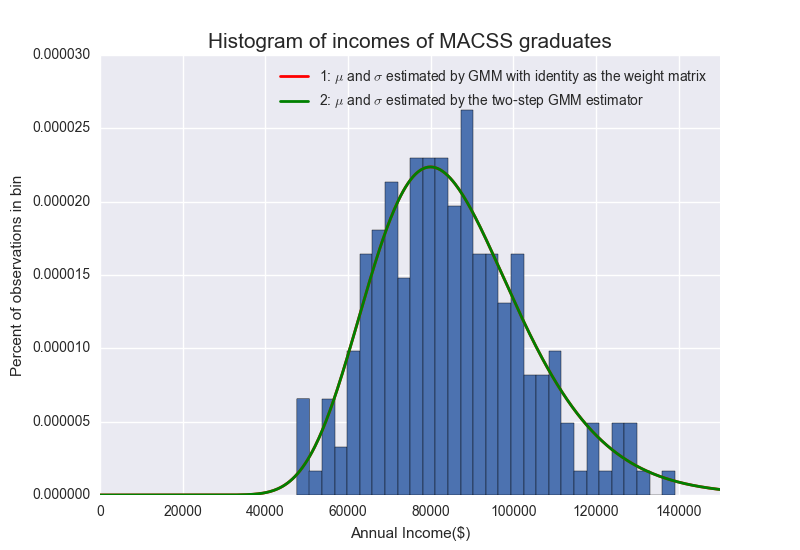
\includegraphics{images/Fig_1c.png}}}
\end{figure}

\noindent\textbf{Problem 2}
In \href{http://proxy.uchicago.edu/login?url=http://search.ebscohost.com/login.aspx?direct=true&db=a9h&AN=117836513&site=eds-live&scope=site}{this study}, the 
authors propose "a weakly supervised framework for domain adaptation in a multi-modal
context for multi-label classification." The methods proposed in this study "
take us a step closer to object recognition in the wild and automatic video 
indexing." The researchers trained the model on a set of training images and
subtitles from nature documentaries to recognize wildlife in said nature 
documentaries.
\\
\\
When thinking about formulating the data collection as a human computation 
project, the data collected is the data being used to train the model.
\\
\\
The authors of the study seem to have used a resource called ImageNet
in order to train their model. In order to provide their model with a greater volume
and diversity of training data, a call could be made for humans to provide images
 of certain animals, with maybe a subset of humans trying to identify animals
from these submissions to help ensure the accuracy of the images provided. I'm
assuming there is a limit to which the size of the training dataset gives better
results, but until that limit is reached, human computation might have been able
to supplement the ImageNet resource the researchers used.
\\
\\
Of course however, this form of human computation in data collection is especially
susceptible to a high number of repeat images, say the first few results for a 
zebra on an image search. It would be nice to incentivize unique content, perhaps
with a small bonus, or providing a screenshot of a video with the requested animal
inside. Even so, according to Michael Franklin, there seem to be a number of people
who try really hard to not submit the same images other people are likely to submit
so there is hope for unique submissions even without incentives.
\\
\\
Lastly, since the authors of the study also utilized the subtitles from the nature 
documentaries that they were training in order to "adapt" their model to their 
testing data. Indeed, their paper focused on how this improved the accuracy of 
their model when compared to simply using ImageNet as a resource. This 
adapatation could be supplemented by human computation. Going back to the 
zebra example, a picture of a zebra from the documentary could be shown and humans
could be asked to describe the image and/or animal in the image without using 
the name of the animal. While humans could provide troll descriptions 
without using the name of the animal, these troll descriptions could be thrown out
if they are shown to not improve the accuracy of the model. One might 
expect "better" descriptions to improve the accuracy of the model in identifying
the animals.

% \noindent\textbf{Part (c).} 
% \begin{figure}[h!]\centering\captionsetup{width=4.0in}
%   \caption{\textbf{1c}}\label{FigExample}
%   \fbox{\resizebox{4.0in}{3.0in}{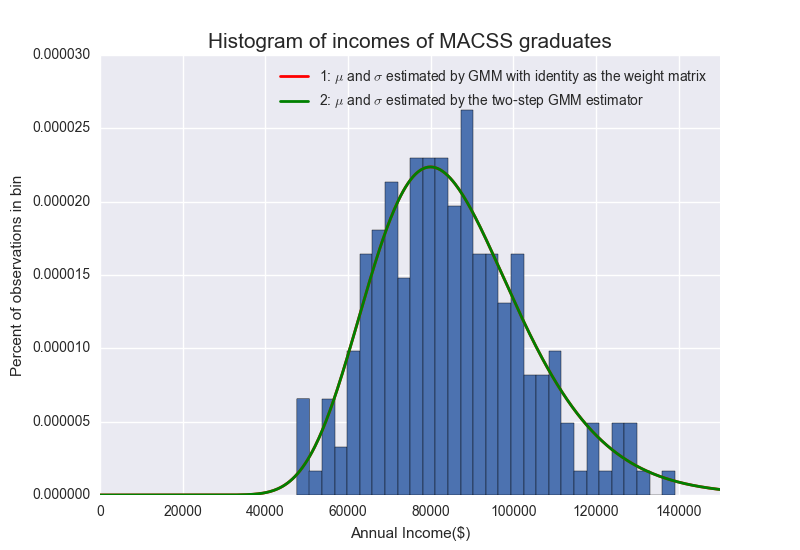
\includegraphics{images/Fig_1c.png}}}
% \end{figure}
% 18.08\% of the time I will be able to pay off the loan in 10 years.

% \noindent\textbf{Part (d).} 
% \begin{figure}[h!]\centering\captionsetup{width=4.0in}
%   \caption{\textbf{1d}}\label{FigExample}
%   \fbox{\resizebox{4.0in}{3.0in}{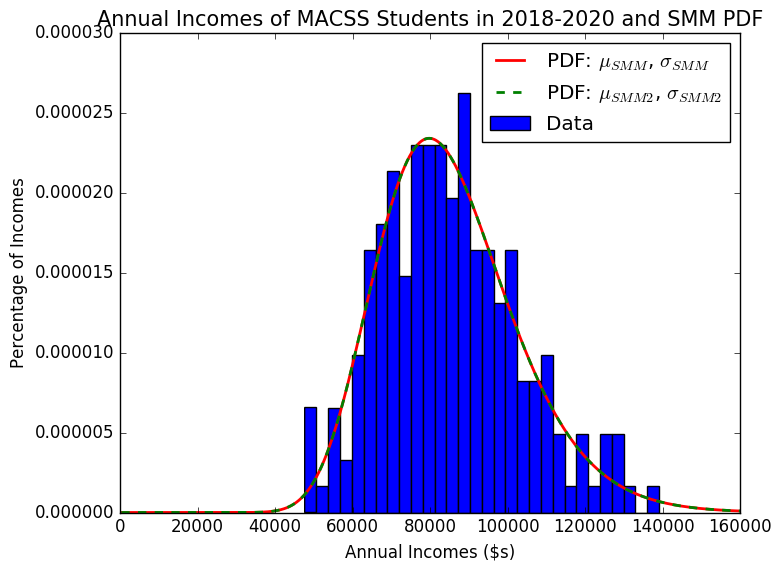
\includegraphics{images/Fig_1d.png}}}
% \end{figure}
% 69.87\% of the time I will be able to pay off the loan in 10 years.
 
% \begin{equation*}
%   \Omega_{j,t} = \left(\frac{\int_{m=4}^\infty(2t + 7m)dm}{\sum_{x=1}^23\sin(\theta_{j,x})}\right) + 7
% \end{equation*}
% You could refer to that object from the equation in math mode $\Omega_{j,t}$ in the sentence. Or if you wanted to talk about the equation, you could remove the asterisks, give it a label, and refer to it with references.
% \begin{equation}\label{EqCoolness}
%   \Omega_{j,t} = \left(\frac{\int_{m=4}^\infty(2t + 7m)dm}{\sum_{x=1}^23\sin(\theta_{j,x})}\right) + 7
% \end{equation}
% Look how cool equation \eqref{EqCoolness} is.

% You might want to include a table in your \LaTeX document. For this, you use the \texttt{tabular} environment.
% \begin{table}[htbp] \centering \captionsetup{width=6.0in}
% \caption{\label{TabExample}\textbf{Sweet example table}}
%   \begin{threeparttable}
%   \begin{tabular}{>{\small}l |>{\small}l >{\small}c |>{\small}r}
%     \hline\hline
%     Degrees & Time to completion & happiness (1-10) & added value (1-10) \\
%     \hline
%     High school diploma & 3.9 years & 5 & 2 \\
%     Bachelor's degree   & 3.8 years & 7 & 5 \\
%     Master's degree     & 1.7 years & 8 & 4 \\
%     PhD                 & 5.7 years & 3 & 7 \\
%     \hline\hline
%   \end{tabular}
%   \begin{tablenotes}
%     \scriptsize{\item[*]With this \texttt{threeparttable} environment, you can add nice subtext to a table.}
%   \end{tablenotes}
%   \end{threeparttable}
% \end{table}
% Lastly, you can add figures to your document. Just make sure that the reference to the figure has the right file path. Figure \ref{FigExample} is pretty nice. But, ideally, you would have something better than a pencil drawing. But you can just place any \texttt{.png} file into the \texttt{includegraphics} command.
% \begin{figure}[htb]\centering\captionsetup{width=4.0in}
%   \caption{\textbf{Great example figure}}\label{FigExample}
%   \fbox{\resizebox{4.0in}{3.0in}{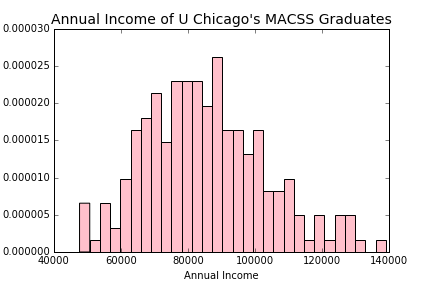
\includegraphics{images/Fig_1a.png}}}
% \end{figure}


\end{document}